% !TeX spellcheck = es_ES
%----------------------------------------------------------------------------------------
%	PACKAGES AND OTHER DOCUMENT CONFIGURATIONS
%----------------------------------------------------------------------------------------

\documentclass[fleqn,10pt]{SelfArx} % Document font size and equations flushed left
%\usepackage{chemmacros}
\usepackage{ifthen}
\usepackage{calc}
\usepackage{microtype}
\usepackage{ifpdf}
\usepackage[utf8]{inputenc}
\usepackage{amsmath, amsfonts, amssymb}
\usepackage{graphicx, xcolor}
\usepackage{booktabs}
\usepackage{fancyhdr}
\usepackage{lastpage}
\usepackage{titlesec}
\usepackage{titletoc}
\usepackage{enumitem}
\usepackage{cuted}
\usepackage[version=3]{mhchem}
\usepackage{lipsum}
\usepackage{graphbox}
\usepackage{cuted}
\usepackage{tabularx}
\usepackage{setspace}
%----------------------------------------------------------------------------------------
%	COLUMNS
%----------------------------------------------------------------------------------------

\setlength{\columnsep}{0.55cm} % Distance between the two columns of text
\setlength{\fboxrule}{1pt} % Width of the border around the abstract

%----------------------------------------------------------------------------------------
%	COLORS
%----------------------------------------------------------------------------------------

\definecolor{color1}{RGB}{0,94,157} % Color of the article title and sections
\definecolor{color2}{RGB}{255,243,210} % Color of the boxes behind the abstract and headings

%----------------------------------------------------------------------------------------
%	HYPERLINKS
%----------------------------------------------------------------------------------------

\usepackage{hyperref} % Required for hyperlinks
\hypersetup{hidelinks,colorlinks,breaklinks=true,urlcolor=color2,citecolor=color1,linkcolor=color1,bookmarksopen=false,pdftitle={Title},pdfauthor={Author}}

%----------------------------------------------------------------------------------------
%	ARTICLE INFORMATION
%----------------------------------------------------------------------------------------

\JournalInfo{L. de Qu\'imica inorg\'anica II, No. 2, 2016-20} % Journal information
%\Archive{Additional note} % Additional notes (e.g. copyright, DOI, review/research article)

\PaperTitle{La separaci\'on de complejos de cromo con el uso de una columna de
intercambio i\'onico} % Article title

\Authors{Juan Barbosa{\color{color1}\textsuperscript{1}\textsuperscript{,2}*},
	Alejandro Camacho{\color{color1}\textsuperscript{1}\textsuperscript{,3}**}} %
%Authors
\affiliation{{\color{color1}\textsuperscript{1}}\textit{Departamento de Qu\'imica, Universidad de los Andes, Bogot\'a, Colombia}} % Author affiliation
\affiliation{{\color{color1}\textsuperscript{2}}\textit{Departamento de F\'isica, Universidad de los Andes, Bogot\'a, Colombia}} % Author affiliation
\affiliation{{\color{color1}\textsuperscript{3}}\textit{Departamento de	F\'isica, Universidad Nacional, Bogot\'a, Colombia}}
\affiliation{{\color{color1}*}\textbf{Email}: js.barbosa10@uniandes.edu.co} %
%Corresponding author
\affiliation{{\color{color1}**}\textbf{Email}: a.camacho10@uniandes.edu.co}
\Keywords{Intercambio i\'onico, cromatograf\'ia, cloruros de cromo, espectroscop\'ia} %
%Keywords - if you don't want any simply remove all the text between the curly
%brackets
\newcommand{\keywordname}{Keywords} % Defines the keywords heading name

%----------------------------------------------------------------------------------------
%	ABSTRACT
%----------------------------------------------------------------------------------------
\Abstract
{
En el presente documento se muestran la s\'intesis de los distintos complejos hidratados del cloruro de cromo (III), y su caracterizaci\'on por espectroscop\'ia UV-vis. Los tres complejos son obtenidos \texit{in situ} al disolver \ce{CrCl_3} en agua. La concentraci\'on de estos depende del tiempo. Los compuestos son separados usando una columna de intercambio i\'onico de caracter cati\'onico, con 3 soluciones distintas de \'acido percl\'orico con concentraciones entre 0.1 M y 4 M como eluyentes.
}
%----------------------------------------------------------------------------------------

\begin{document}
	\flushbottom % Makes all text pages the same height
	\maketitle % Print the title and abstract box
	%\tableofcontents % Print the contents section
	\thispagestyle{empty} % Removes page numbering from the first page
	%----------------------------------------------------------------------------------------
	%	ARTICLE CONTENTS
	%----------------------------------------------------------------------------------------
	\section*{Introducci\'on}
	Existen una gran diversidad de mol\'eculas que pueden llevar a cabo intercambio de iones en soluci\'on. Este fen\'omeno fue descubierto en 1850 por Thompson y Way, los cuales notaron que los iones de amonio en soluci\'on pod\'ian ser sustituidos con facilidad por iones de calcio luego de pasar la soluci\'on a trav\'es de un tubo con tierra en su interior. Cincuenta y cinco a\~nos despu\'es el mismo principio fue usado para reducir la cantidad de iones Mg(II) y Ca(II) en el agua \cite{Chen}. La primera publicación científica relacionada con la cromatografía de iones se dio en septiembre del año 1975 demostrando que usando una resina adecuada para la retención de cationes y otra para la retención de aniones el eluyente perdía su conductividad, relacionando esta ultima, con la detección muy sensitiva de iones en solución. Antes la detección de iones se encontraba condicionada a la fotometría, la fluorencia y las medidas electroquímicas, abriendo esta nueva técnica las puertas al análisis de múltiples muestras clínicas \cite{ion}.    
	
	Con el objetivo de hacer el intercambio m\'as eficiente, los procesos fueron enfocados a interacciones liquido-s\'olido. En la fase l\'iquida se encuentran las especies i\'onicas a separar, las cuales al interactuar con una resina son retenidas, mientras otros iones son liberados dando lugar a una fase l\'iquida con naturaleza qu\'imica distinta. Los primeros s\'olidos usados fueron rocas de zeolita, mineral poroso con alto contenido de aluminosilicatos. Sin embargo la aplicaci\'on de la zeolita como intercambiador i\'onico era limitada, debido a su poca estabilidad en medios \'acidos \cite{Chen}.
	\begin{scheme}[h]
	    \centering
	    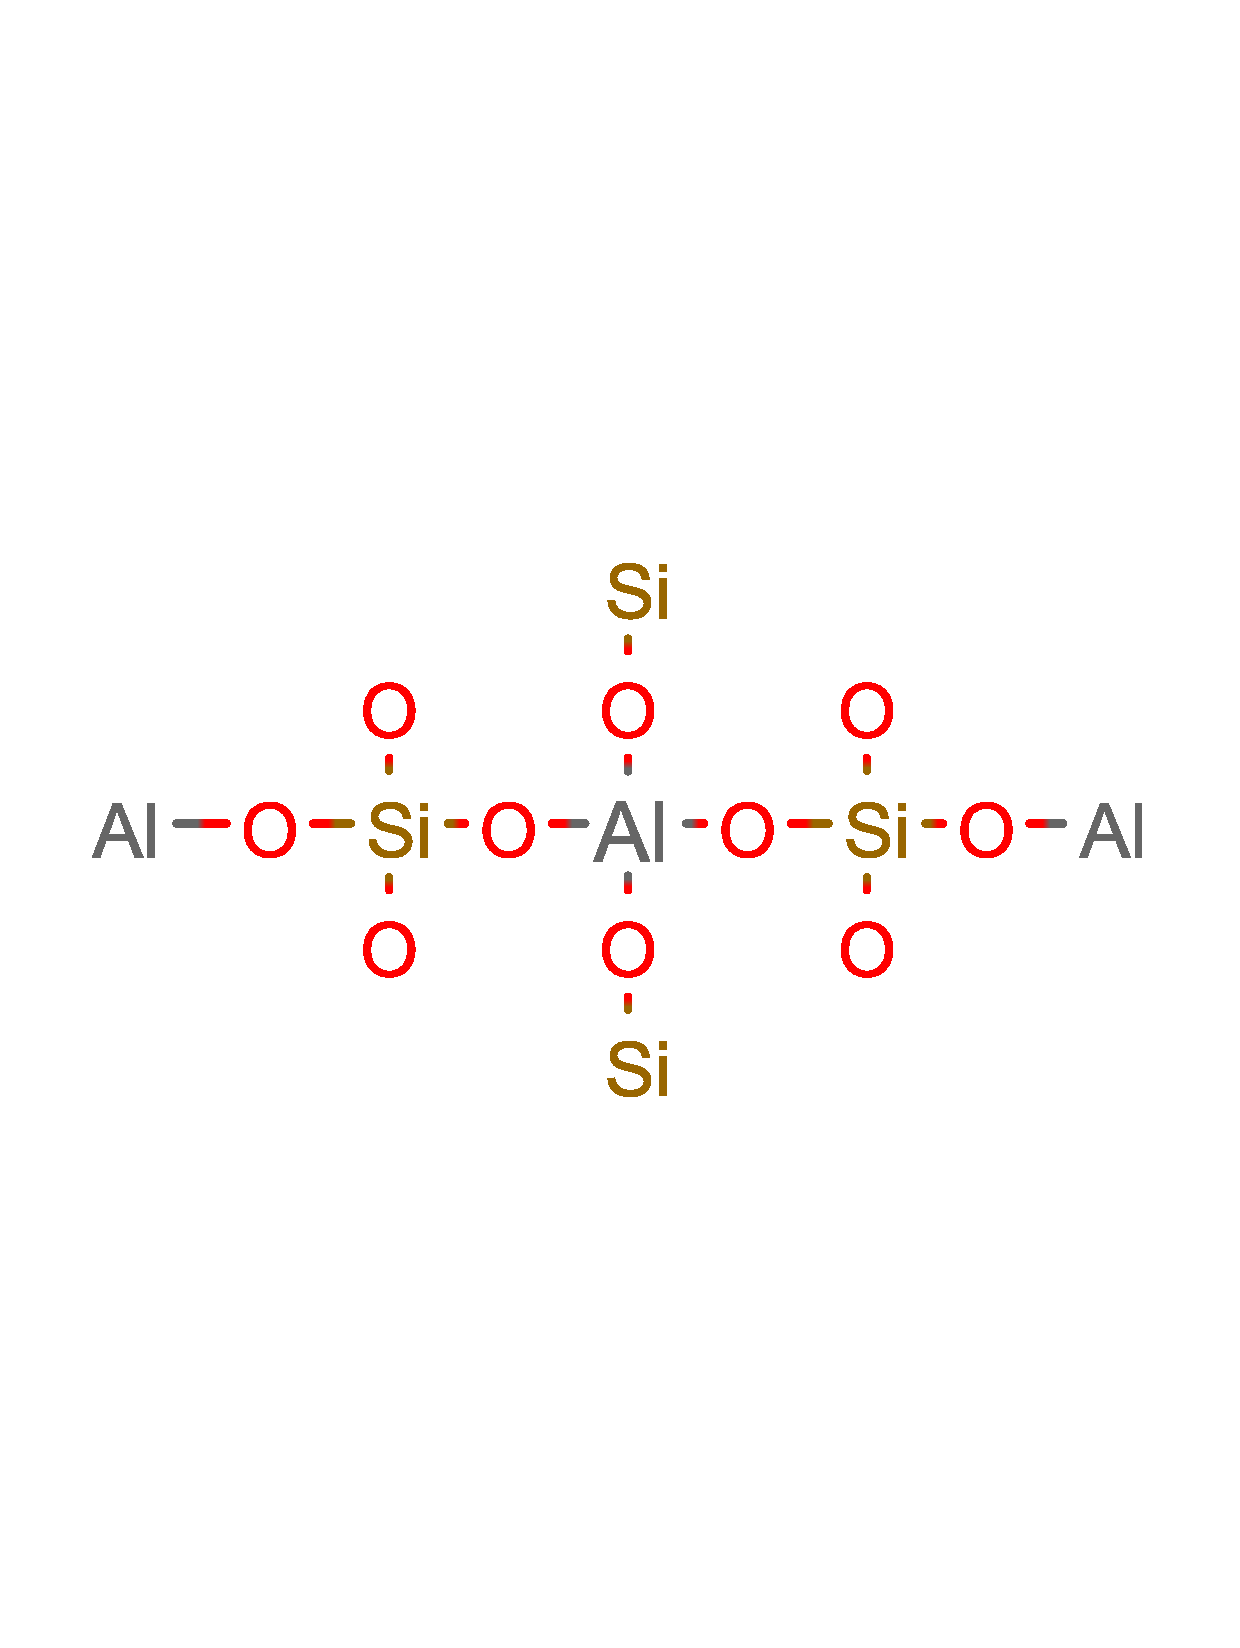
\includegraphics[scale=0.2]{images/Zeolite.pdf}
	    \caption{Estructura principal de la zeolita, construida a partir de \ce{AlO4^{-5}} y \ce{SiO4^{-4}} tetra\'edricos.}
	    \label{sch:zeolita}
	\end{scheme}
	
	La soluci\'on propuesta fueron resinas sint\'eticas. En un inicio pol\'imeros de metanal y derivados de aminas arom\'aticas. Para los a\~nos 50 la mayor\'ia de las resinas consist\'ian en pol\'imeros de poliestireno \cite{Chen}. La resina usada en este experimento es un copol\'imero de estireno y divinilbenceno, al cual se le han agregado grupos bisulfitos, permitiendo el intercambio de especies cat\'ionicas \cite{DOWEX}. 
	\begin{scheme}[h]
	    \centering
	    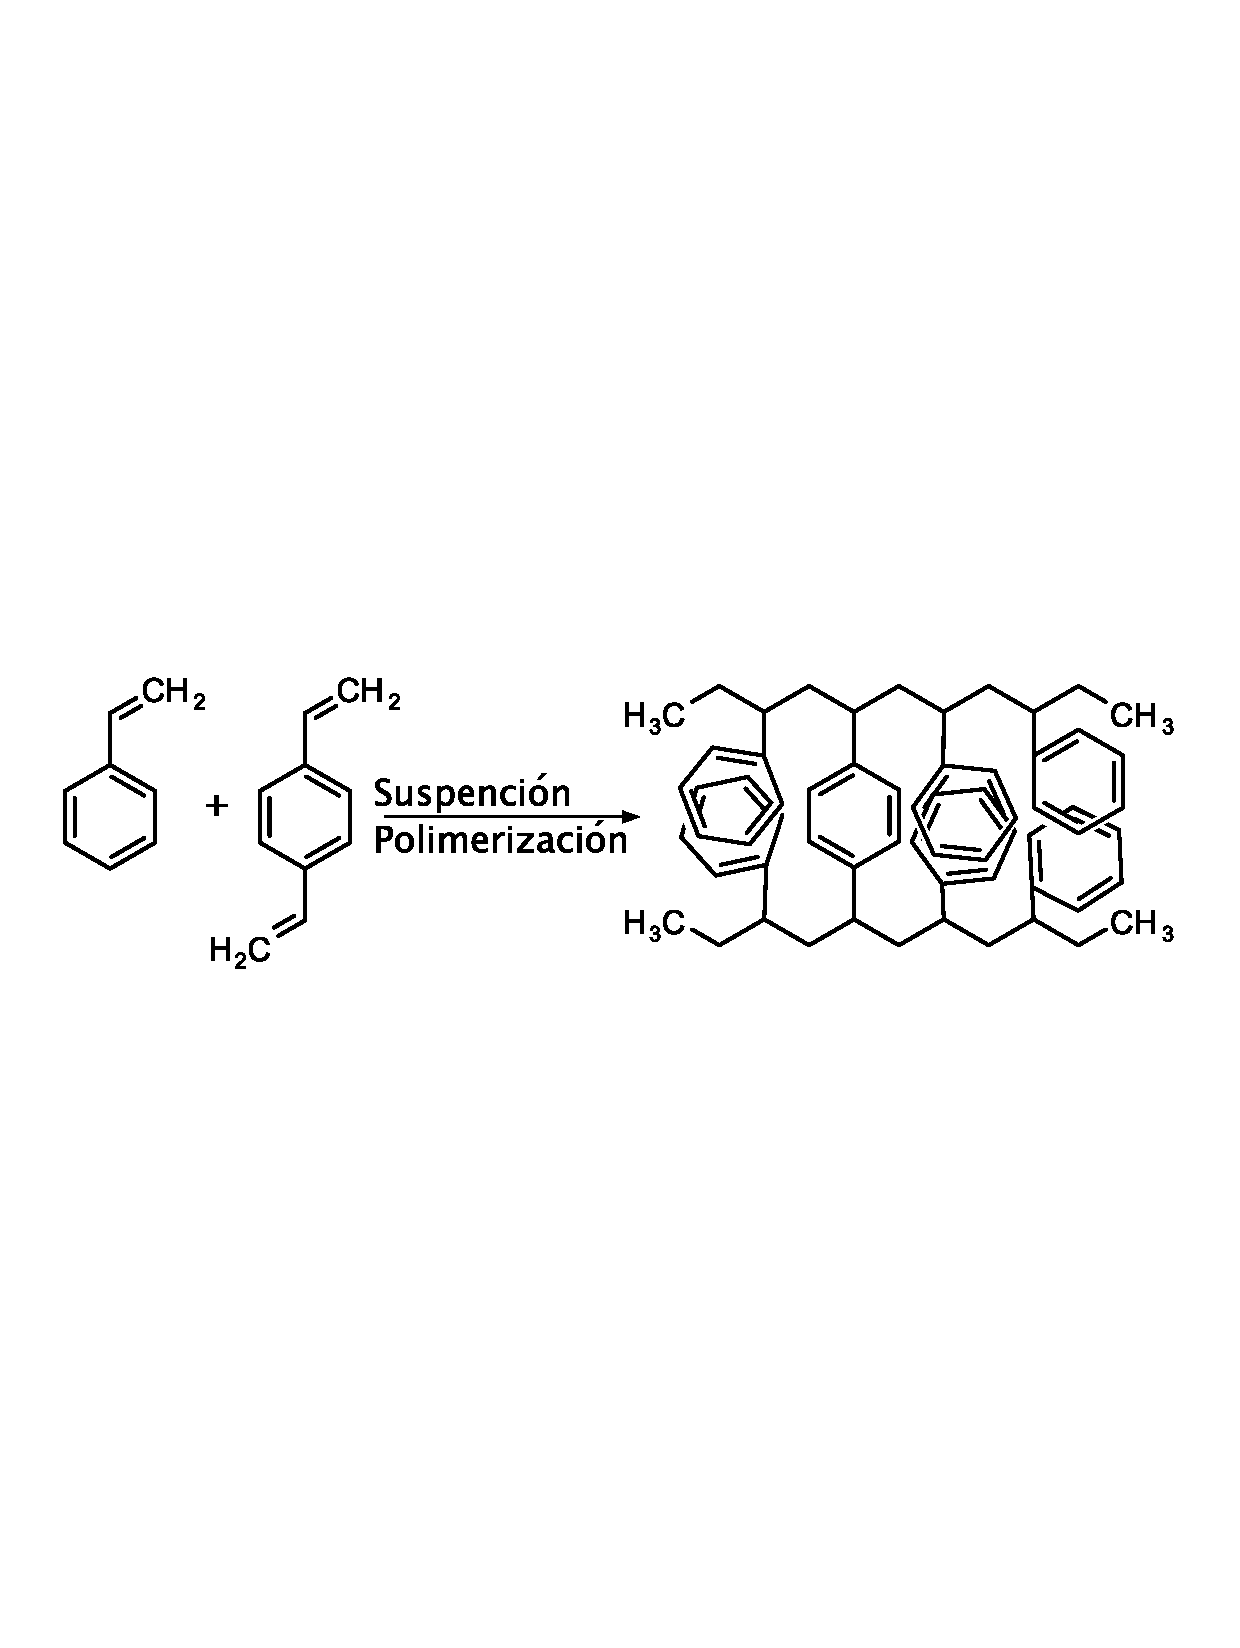
\includegraphics[width=\linewidth]{images/Resina.pdf}
	    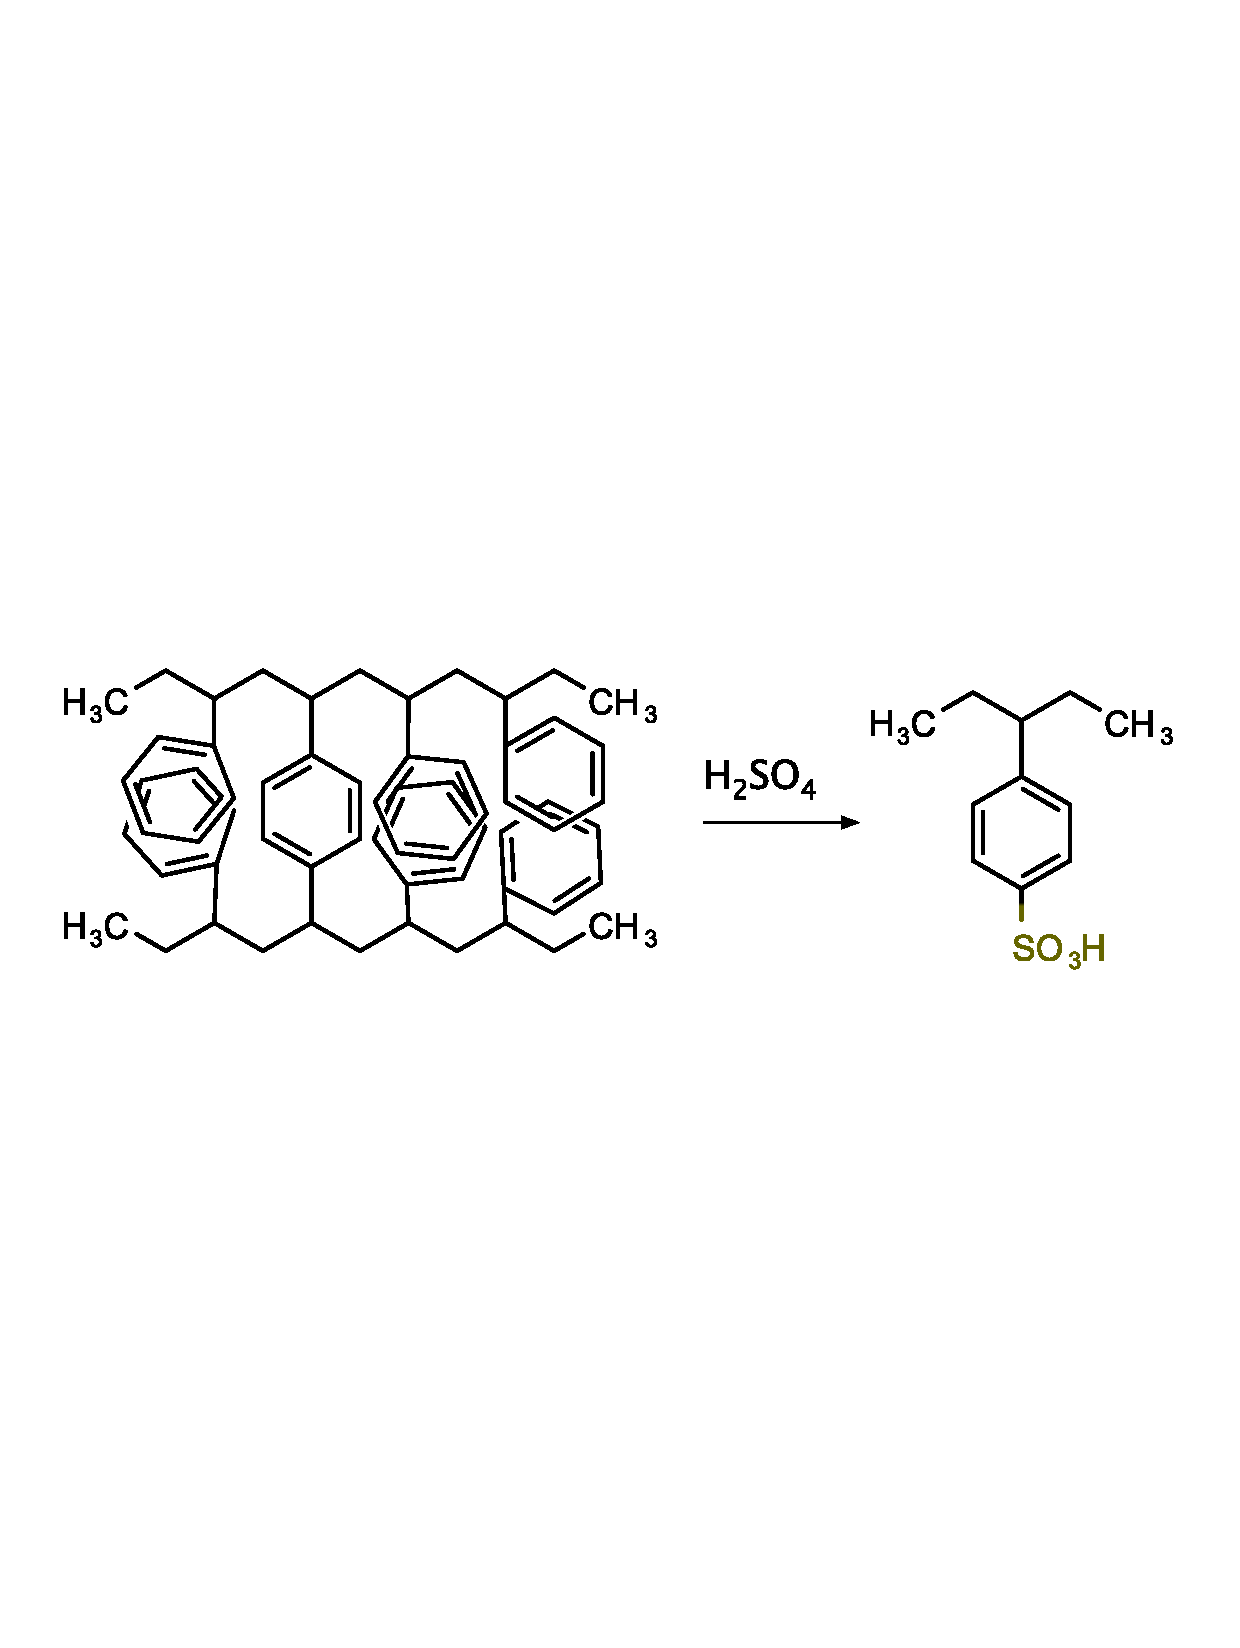
\includegraphics[width=\linewidth]{images/Resina2.pdf}
	    \caption{S\'intesis de la resina DOWEX 50WX8 \cite{DOWEX}.}
	    \label{sch:DOWEX}
	\end{scheme}
	
	Lo anterior teniendo en cuenta que el hidr\'ogeno del sulfito es f\'acilmente reemplazado por un cati\'on inorg\'anico. Este proceso se repite permanentemente dando lugar a un equilibrio din\'amica para las especies en la resina.
	\begin{equation}
	\ce{RSO3^-H+ + M+ <=> RSO3^-M+ + H+}
	\end{equation}
	
	En este caso los cationes corresponden con los complejos hidratados del cloruro de cromo (III). Los complejos se muestran en el \autoref{sch:complexes}, en donde se puede observar como cambia la carga del complejo. Lo anterior constituye un papel fundamental en la forma como interact\'ua con la resina.
	\begin{scheme}[h]
	    \centering
	    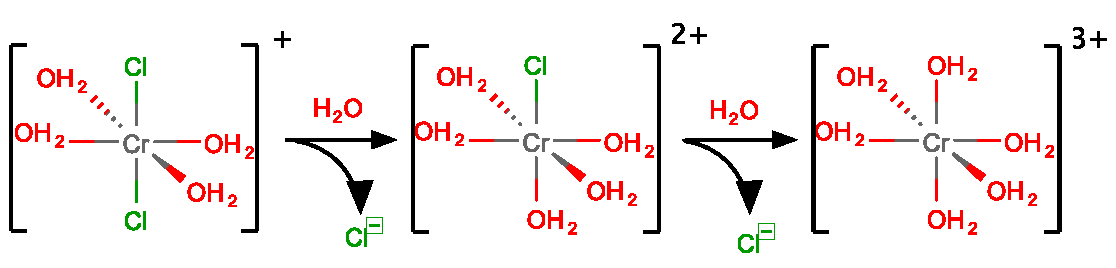
\includegraphics[width=\linewidth]{images/Complex.pdf}
	    \caption{Complejos de cromo a separar.}
	    \label{sch:complexes}
	\end{scheme}
	
	Adicionalmente los complejos en el \autoref{sch:complexes} presentan esferas de coordinaci\'on totalmente distintas, raz\'on por la cual existe un espectro UV-vis caracter\'istico para cada especie permitiendo que se identifique el complejo en solución y se cuantifique.
	
	\section{Metodolog\'ia}
	La realizaci\'on del experimento tuvo lugar en 3 etapas distintas. En primer lugar, la columna fue prepara en l\'iquido usando una relaci\'on 2/3 agua resina Dowex 50WX8. La altura de la columna fue de 10 cm aproximadamente. La columna se lava constantemente con agua hasta lograr que esta eluya sin coloraci\'on. Tres soluciones de \'acido percl\'orico con concentraciones de 0.1 M, 1.0 M y 4.0 M fueron preparadas en un volumen de 100 mL. Posteriormente fue preparada una soluci\'on 0.35 M de cromo (III) aforando 2.33 g de \ce{CrCl3.H2O} en 25 mL de agua.
	
	\begin{scheme}[h]
	    \centering
	    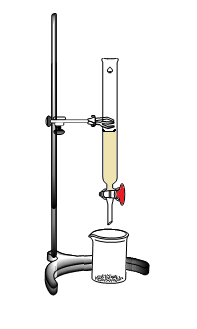
\includegraphics[scale=0.7]{images/montaje.png}
	    \caption{Montaje experimental para la separación de los iones.}
	    \label{sch:montaje}
	\end{scheme}
	
	La segunda etapa consiste en la caracterizaci\'on de los distintos iones de cromo en la \autoref{sch:complexes}, para el primero se vierten 2.5 mL de la soluci\'on previamente preparada en la columna, y se eluye con una soluci\'on \ce{HClO4} 0.1 M. La fracci\'on con mayor coloraci\'on es analizada usando un espectrofot\'ometro y cubetas de pl\'astico. Para el ion cloropentaacuocromo(III) se calientan 2.5 mL de la soluci\'on inicial de Cr(III) sobre un beaker con agua en ebullici\'on por cerca de 3 minutos, posteriormente este se disuelve en 2.5 mL de agua y se agregan a la columna. En el caso del complejo hexaacuo, 2.5 mL la soluci\'on de Cr(III) son adicionados a 2.5 mL de agua y se deja hervir la soluci\'on por 5 minutos.
	
	El \'ultimo procedimiento consiste en la separaci\'on de los tres iones presentes, usando la columna en gradiente de concentraci\'on. En todos los casos se obtienen los espectros UV-vis de los complejos. 
	
	\section{Resultados y Discusi\'on}
	
	Se realizo la elución consecutiva con las soluciones a diferente concentración de ácido perclorico, esto debido a la acidez característica del metal, tomando una alicuota de cada elución para medir la absorbancia e identificar las longitudes de onda en que se presenta mayor absorción, aprovechando así los cambios en la esfera interna de coordinación del complejo de cromo, pretendiendo con la medida identificar y cuantificar el complejo eluido y su proporción.
	
\begin{table}[h]
\centering
\caption{Tabla de resultados: se presentan las longitudes de mayor absorción y el valor de absorbancia para la medida de ls tres complejos extraídos \ce{c_{1}}, \ce{c_{2}} y \ce{c_{3}} con sus respectivas replicas si se realizaron.}\\

\label{t1}
\\
\begin{tabular}{c|cccc}
\hline
\textbf{Complejo} & $\lambda_{1}$ & A$_{1}$ & $\lambda_{1}$  & A$_{2}$ \\\hline
c$_1$ & 637.0 &0.336  &448.0  &0.302  \\
R c$_1$& 637.0 &0.615  &448.0  &0.552  \\
c$_2$ & 610.0 &0.277  &430.0  &0.351  \\\
R c$_2$& 610.0 &0.222  &430.0  &0.522  \\
c$_3$ & 604.0 &0.299  &415.0  &0.190  \\\hline
\end{tabular}
\end{table}

Se pueden hacer dos consideraciones en relación a la estabilidad de los complejos de cromo a separar \autoref{sch:complexes}, y es que en la medida en que los ligandos presentes en la esfera interna del complejo tengan el mismo entorno químico y las mismas propiedades, el sistema logrará alcanzar una mejor distribución espacial y por tanto una mayor estabilidad cuando menos en la esfera interna, reduciendo esto la tensión, las interacciones entre ligandos y la energía del complejo implicando que la estabilidad sea:

\small
\begin{equation}\label{eq:complexesStabilities}
\ce{[Cr(H_{2}O)_{6}]^{+3}>[CrCl(H_{2}O)_{5}]^{+2}>[CrCl_{2}(H_{2}O)_{4}]^{+1}}    
\end{equation}
\normalsize

Relación que se hace evidente en la longitud de onda absorbida \autoref{t1}, pues se necesitan ondas con menor longitud, es decir, mas energéticas para hacer vibrar o absorber el complejo \ce{[Cr(H_{2}O)_{6}]^{+3}} con relación a \ce{[CrCl(H_{2}O)_{5}]^{+2}} y mas energ\'eticas para hacer vibrar o absorber a \ce{[CrCl(H_{2}O)_{5}]^{+2}} con relación a \ce{[CrCl_{2}(H_{2}O)_{4}]^{+1}} mostrando que los enlaces son mas fuertes y estables en el ion \ce{[Cr(H_{2}O)_{6}]^{+3}}.

Adicionalmente se nota durante la practica que el complejo \ce{[CrCl_{2}(H_{2}O)_{4}]^{+1}} tiene un color verde oscuro, el complejo \ce{[CrCl(H_{2}O)_{5}]^{+2}} verde claro y el ultimo complejo \ce{[Cr(H_{2}O)_{6}]^{+3}} es un violeta muy fuerte.

El segundo aspecto que se puede considerar en relación a  los complejos de \ce{Cr^{+3}}, más allá de la estabilidad es espontaneidad presente, que provoca el intercambio de los iones cloruro por el agua, apoyado lo anterior por los estudios realizados en el año de 1957 por K. Schug y E. King \cite{KE} con miras a medir el $\Delta$H del intercambio de ligando a una temperatura y fuerza iónica definida, concluyendo que la entalpía se hace cada vez menor y negativa a medida que se intercambian iones cloruros por agua en la esfera interna de coordinación.
Sin embargo para asegurar la espontaneidad de la reacción y en ultimas que se alcance el equilibrio para la concentración de los iones, donde se debe encontrar gran cantidad de iones \ce{[Cr(H_{2}O)_{6}]^{+3}} se debe considerar el efecto que tiene la liberación de iones cloruro a la matriz, aumentando la fuerza iónica y la interacción eléctrica, cuyo efecto puede llegar a tener una entropía negativa. Aun así se debe considerar que el sistema es abierto y tiene constante adición de ácido completamente disociable (ácido percl\'orico) a altas concentraciones por lo que se puede asumir que el efecto del intercambio de un cloruro (cargado) por una molécula de agua (neutra) no es significativo en comparación.

En la segunda etapa de la experiencia se siembran en la columna \ce{3 mL} de la solución preparada y se obtienen los siguientes resultados.

\begin{table}[h!]
\centering
\caption{Resultados de la separaci\'on de los iones.}
\begin{tabular}{c|cccc}
\hline
\textbf{Complejo} & \ce{\lambda_{1}} & \ce{A_{1}}  &\ce{\lambda_{1}}  & A_{2} \\\hline
c$_1$ & 610.0  & 0.159  & 430.0 &0.204 \\
c$_2$ & 607.0 &0.137  &430.0  & 0.171 \\
R c$_2$& 607.0 & 0.132& 430.0 &0.164 \\
c$_3$ & 580.0 &0.151 &410.0  &0.204 \\\hline
\end{tabular}
\label{t1}
\end{table}

Donde se ve el desplazamiento del ion más inestable \ce{[CrCl_{2}(H_{2}O)_{4}]^{+1}} a  \ce{[CrCl(H_{2}O)_{5}]^{+2}} debido al paso del tiempo.

Adicionalmente la diferencia entre las medidas esperadas y las obtenidas se puede deber a diferencias en la calibración de los equipos utilizados para la medici\'on.
	
	\section{Preguntas}
	
	\begin{itemize}
	    \item Esta reacción de intercambio de ligandos es catalizada por el ultimo ión ya que la presencia u ausencia de este permite que el intercambio ocurra directamente sobre la esfera interna de coordinación produciendo un intermediario binuclear donde un atomo de cromo se encuentra en estado de oxidación (III) y el otro en estado (II), dada la versatilidad del cromo como metal de transición.
	    \\
	    \begin{equation}
	        \begin{array}{l}
	             \ce{(H_{2}O)_{5}Cr^{(III)}ClCr^{(II)}(OH_{2})_{5}^{+4} ->} \\
	            \ce{(H_{2}O)_{5}Cr^{(II)}ClCr^{(III)}(OH_{2})_{5}^{+4}}
	        \end{array}
	   \end{equation}
	   \\
	   \begin{equation}
            \begin{array}{l}
	            \ce{CrCl(OH_{2})_{5}^{+2} + Cr(OH_{2})_{6}^{+2} ->}\\
	            \ce{Cr(OH_{2})_{6}^{+2} + CrCl(OH_{2})_{5}^{+2}}
	        \end{array}
	    \end{equation}

	    \item Dependiendo la concentración de iones cloruros en la matriz este paso puede llegar a ser determinante en la cinética de reacción así pues al tener ion mercurio en solución se favorece debido a la precipitación de la sal \ce{HgCl_{2}} que desplaza el equilibrio hacia el remplazo del ion cloruro en la esfera interna de coordinación por una molécula de agua.
	    \item Se puede utilizar la columna de intercambio iónico con una resina que permita ya no la retención de especies cationicas sino anionicas, utilizando una sustancia básica, optimizando la concentración para que la sustancia sea mas básica que el compuesto a eluir y mas ácida que el compuesto a retener. Además se debe considerar la estabilidad en solución de la sustancia o el equilibrio presente entre lo iones a separar. 
	    \item Se sabe que los complejos de cromo son sustancias en solución son bastante ácidas por la deficiencia de electrones del centro metálico,por lo que es hace falta un ácido fuerte para que estos actúen como bases.
	    \item Se utiliza el estudio UV-vis en lugar de IR porque no solo es un análisis mas sencillo y rápido, sin necesidad de separar el solido o incluir la solución en una celda resistente a la acción del ácido, que no interfiera sino que los picos de absorción que se identifican en UV-vis son suficientes para la identificación de los complejos. Además no se dispone de IR.
	\end{itemize}

	\section{Conclusiones}
	El éxito en la extracción depende de la estabilidad de los iones involucrados, de la resina utilizada y su capacidad de retención y de la identificación del pH adecuado para realizar la extracción. Como se discuti\'o anteriormente la concentraci\'on de los complejos de cromo tiende hacia el hexaacuo como se observa en la \autoref{eq:complexesStabilities}, debido a la duraci\'on de tres semanas del experimento, no fue posible establecer con claridad la concentraci\'on de los mismos, y se aplic\'o como criterio de an\'alisis la longitud de onda de m\'axima absorci\'on de cada complejo.
	\phantomsection
	\bibliographystyle{unsrt}
	\begin{thebibliography}{9}
	    \bibitem{Chen}
	    Chan, J. Paul; Yang, L.; Wang, L. K.; Thong, S. \textit{Advaned Physicochemical Treatment Processes}; Humana Press: Totowa, NJ, 2006. 
	    \bibitem{ion}
	    \texit{Roy Wetzel, Pohl C, Riviello J. Ion chromatography. In: Macdonald J, editor. Inorganic Chromatogtaphic Analysis. New York: John Wiley & Sons, Inc.; 1985. p. 450.}
		\bibitem{DOWEX}
		DOWEX. \texit{Fine Mesh Spherical Ion Exchange Resins}; DoW Water Solutions.
		\bibitem{KE}
		\texit{Schung K, King E. A calorimetric determination of the values of DH for certain Chrmium (III)-Chloride complex ion reactions. Am Chem Soc. 1957;3. }
	\end{thebibliography}
\end{document}
